%%%%%%%%%%%%%%%%%%%%%%%%%%%%%%%%%%%%%%%%%
% The Legrand Orange Book
% LaTeX Template
% Version 1.1 (11/4/13)
%
% This template has been downloaded from:
% http://www.LaTeXTemplates.com
%
% Original author:
% Mathias Legrand (legrand.mathias@gmail.com)
%
% License:
% CC BY-NC-SA 3.0 (http://creativecommons.org/licenses/by-nc-sa/3.0/)
%
% Compiling this template:
% This template uses biber for its bibliography and makeindex for its index.
% This means that to update the bibliography and index in this template you
% will need to run the following sequence of commands in the template
% directory:
%
% 1) pdflatex main
% 2) makeindex main.idx -s StyleInd.ist
% 3) biber main
% 4) pdflatex main
%
% This template also uses a number of packages which may need to be
% updated to the newest versions for the template to compile. It is strongly
% recommended you update your LaTeX distribution if you have any
% compilation errors.
%
% Important note:
% Chapter heading images should have a 2:1 width:height ratio,
% e.g. 920px width and 460px height.
%
%%%%%%%%%%%%%%%%%%%%%%%%%%%%%%%%%%%%%%%%%

%----------------------------------------------------------------------------------------
%	PACKAGES AND OTHER DOCUMENT CONFIGURATIONS
%----------------------------------------------------------------------------------------

\documentclass[11pt,fleqn]{book} % Default font size and left-justified equations

\usepackage[top=3cm,bottom=3cm,left=3.2cm,right=3.2cm,headsep=10pt,a4paper]{geometry} % Page margins

\usepackage{xcolor} % Required for specifying colors by name
\definecolor{ocre}{RGB}{243,102,25} % Define the orange color used for highlighting throughout the book

% Font Settings
\usepackage{avant} % Use the Avantgarde font for headings
%\usepackage{times} % Use the Times font for headings
\usepackage{mathptmx} % Use the Adobe Times Roman as the default text font together with math symbols from the Sym­bol, Chancery and Com­puter Modern fonts
\usepackage{microtype} % Slightly tweak font spacing for aesthetics
\usepackage[utf8]{inputenc} % Required for including letters with accents
\usepackage[T1]{fontenc} % Use 8-bit encoding that has 256 glyphs

% Bibliography
%\usepackage{hyperref} %added by GTG
\usepackage{csquotes} %added by GTG
\usepackage[sorting=nyt,sortcites=true,autopunct=true,babel=hyphen,hyperref=true,abbreviate=false,backend=biber]{biblatex} %style=alphabetic,backref=true,
\addbibresource{bibliography.bib} % BibTeX bibliography file
\defbibheading{bibempty}{}

% Index
\usepackage{calc} % For simpler calculation - used for spacing the index letter headings correctly
\usepackage{makeidx} % Required to make an index
\makeindex % Tells LaTeX to create the files required for indexing

% added by GTG
\usepackage{verbatim}
\usepackage{parskip}
\usepackage{enumitem}
\usepackage{changepage}
\usepackage[official]{eurosym}
\usepackage[lofdepth,lotdepth]{subfig}
\def\numversion{2.3}
\def\svnversion{R1024}

%----------------------------------------------------------------------------------------

%----------------------------------------------------------------------------------------
%	VARIOUS REQUIRED PACKAGES
%----------------------------------------------------------------------------------------

\usepackage{titlesec} % Allows customization of titles

\usepackage{graphicx} % Required for including pictures
\graphicspath{{./Pictures/}} % Specifies the directory where pictures are stored

\usepackage{lipsum} % Inserts dummy text

\usepackage{tikz} % Required for drawing custom shapes

\usepackage[english]{babel} % English language/hyphenation

\usepackage{enumitem} % Customize lists
\setlist{nolistsep} % Reduce spacing between bullet points and numbered lists

\usepackage{booktabs} % Required for nicer horizontal rules in tables

\usepackage{eso-pic} % Required for specifying an image background in the title page

%----------------------------------------------------------------------------------------
%	MAIN TABLE OF CONTENTS
%----------------------------------------------------------------------------------------

\usepackage{titletoc} % Required for manipulating the table of contents

\contentsmargin{0cm} % Removes the default margin
% Chapter text styling
\titlecontents{chapter}[1.25cm] % Indentation
{\addvspace{15pt}\large\sffamily\bfseries} % Spacing and font options for chapters
{\color{ocre!60}\contentslabel[\Large\thecontentslabel]{1.25cm}\color{ocre}} % Chapter number
{}  
{\color{ocre!60}\normalsize\sffamily\bfseries\;\titlerule*[.5pc]{.}\;\thecontentspage} % Page number
% Section text styling
\titlecontents{section}[1.25cm] % Indentation
{\addvspace{5pt}\sffamily\bfseries} % Spacing and font options for sections
{\contentslabel[\thecontentslabel]{1.25cm}} % Section number
{}
{\sffamily\hfill\color{black}\thecontentspage} % Page number
[]
% Subsection text styling
\titlecontents{subsection}[1.25cm] % Indentation
{\addvspace{1pt}\sffamily\small} % Spacing and font options for subsections
{\contentslabel[\thecontentslabel]{1.25cm}} % Subsection number
{}
{\sffamily\;\titlerule*[.5pc]{.}\;\thecontentspage} % Page number
[] 

%----------------------------------------------------------------------------------------
%	MINI TABLE OF CONTENTS IN CHAPTER HEADS
%----------------------------------------------------------------------------------------

% Section text styling
\titlecontents{lsection}[0em] % Indendating
{\footnotesize\sffamily} % Font settings
{}
{}
{}

% Subsection text styling
\titlecontents{lsubsection}[.5em] % Indentation
{\normalfont\footnotesize\sffamily} % Font settings
{}
{}
{}
 
%----------------------------------------------------------------------------------------
%	PAGE HEADERS
%----------------------------------------------------------------------------------------

\usepackage{fancyhdr} % Required for header and footer configuration

\pagestyle{fancy}
\renewcommand{\chaptermark}[1]{\markboth{\sffamily\normalsize\bfseries #1}{}} % Chapter text font settings
\renewcommand{\sectionmark}[1]{\markright{\sffamily\normalsize\thesection\hspace{5pt}#1}{}} % Section text font settings
\fancyhf{} \fancyhead[LE,RO]{\sffamily\normalsize\thepage} % Font setting for the page number in the header
\fancyhead[LO]{\rightmark} % Print the nearest section name on the left side of odd pages
\fancyhead[RE]{\leftmark} % Print the current chapter name on the right side of even pages
\renewcommand{\headrulewidth}{0.5pt} % Width of the rule under the header
\addtolength{\headheight}{2.5pt} % Increase the spacing around the header slightly
\renewcommand{\footrulewidth}{0pt} % Removes the rule in the footer
\fancypagestyle{plain}{\fancyhead{}\renewcommand{\headrulewidth}{0pt}} % Style for when a plain pagestyle is specified

% Removes the header from odd empty pages at the end of chapters
\makeatletter
\renewcommand{\cleardoublepage}{
\clearpage\ifodd\c@page\else\hbox{}
\vspace*{\fill}
\thispagestyle{empty}
\newpage
\fi}

%----------------------------------------------------------------------------------------
%	THEOREM STYLES
%----------------------------------------------------------------------------------------

\usepackage{amsmath,amsfonts,amssymb,amsthm} % For including math equations, theorems, symbols, etc

%\newcommand{\intoo}[2]{\mathopen{]}#1\,;#2\mathclose{[}}
\newcommand{\ud}{\mathop{\,\mathrm{{}d}}\mathopen{}}
%\newcommand{\intff}[2]{\mathopen{[}#1\,;#2\mathclose{]}}
\newtheorem{notation}{Notation}[chapter]

\newtheoremstyle{ocrenum} % Theorem style name
{7pt} % Space above
{7pt} % Space below
{\normalfont} % Body font
{} % Indent amount
{\small\bf\sffamily\color{ocre}} % Theorem head font
{\;\;} % Punctuation after theorem head
{0.25em} % Space after theorem head
{\small\sffamily\color{ocre}\thmname{#1}\thmnumber{\@ifnotempty{#1}{ }\@upn{#2}} % Theorem text (e.g. Theorem 2.1)
\thmnote{\ {\the\thm@notefont\sffamily\bfseries\color{black}--- #3.}}} % Optional theorem note
%\renewcommand{\qedsymbol}{$\blacksquare$} % Optional qed square
\renewenvironment{proof}{{\small\bf\sffamily Proof.}}{\qed}

\newtheoremstyle{blacknumex} % Theorem style name
{7pt} % Space above
{7pt} % Space below
{\normalfont} % Body font
{} % Indent amount
{\small\bf\sffamily} % Theorem head font
{\;\;} % Punctuation after theorem head
{0.25em} % Space after theorem head
{\small\sffamily{\tiny\ensuremath{\blacksquare}}\ \thmname{#1}\thmnumber{\@ifnotempty{#1}{ }\@upn{#2}} % Theorem text (e.g. Theorem 2.1)
\thmnote{\ {\the\thm@notefont\sffamily\bfseries--- #3.}}} % Optional theorem note

\newtheoremstyle{blacknum} % Theorem style name
{7pt} % Space above
{7pt} % Space below
{\normalfont} % Body font
{} % Indent amount
{\small\bf\sffamily} % Theorem head font
{\;\;} % Punctuation after theorem head
{0.25em} % Space after theorem head
{\small\sffamily\thmname{#1}\thmnumber{\@ifnotempty{#1}{ }\@upn{#2}} % Theorem text (e.g. Theorem 2.1)
\thmnote{\ {\the\thm@notefont\sffamily\bfseries--- #3.}}} % Optional theorem note
\makeatother

% Defines the theorem text style for each type of theorem to one of the three styles above
\theoremstyle{ocrenum}
\newtheorem{definitionT}{Definition}[chapter]
\newtheorem{theoremeT}{Theorem}[chapter]
\newtheorem{propositionT}{Proposition}[chapter]
\newtheorem{corollaryT}{Corollary}[chapter]
\theoremstyle{blacknumex}
\theoremstyle{blacknum}
\newtheorem{algorithmT}{Algorithm}[chapter]
\newtheorem{exampleT}{Example}[chapter]

%----------------------------------------------------------------------------------------
%	DEFINITION OF COLORED BOXES
%----------------------------------------------------------------------------------------

\RequirePackage[framemethod=default]{mdframed} % Required for creating the definition, theorem, proposition and corollary boxes

% Definition box
\newmdenv[skipabove=10pt,
skipbelow=7pt,
backgroundcolor=ocre!5,
linecolor=ocre,
innerleftmargin=5pt,
innerrightmargin=5pt,
innertopmargin=5pt,
innerbottommargin=5pt,
leftmargin=0cm,
rightmargin=0cm]{dBox}

% Theorem box
\newmdenv[skipabove=10pt,
skipbelow=7pt,
rightline=false,
leftline=true,
topline=false,
bottomline=false,
linecolor=ocre,
backgroundcolor=ocre!5,
innerleftmargin=5pt,
innerrightmargin=5pt,
innertopmargin=5pt,
innerbottommargin=5pt,
leftmargin=0cm,
rightmargin=0cm,
linewidth=4pt]{tBox}

% Proposition box
\newmdenv[skipabove=10pt,
skipbelow=7pt,
rightline=false,
leftline=true,
topline=false,
bottomline=false,
linecolor=ocre,
backgroundcolor=ocre!5,
innerleftmargin=5pt,
innerrightmargin=5pt,
innertopmargin=5pt,
innerbottommargin=5pt,
leftmargin=0cm,
rightmargin=0cm,
linewidth=4pt]{pBox}

% Corollary box
\newmdenv[skipabove=10pt,
skipbelow=7pt,
rightline=false,
leftline=true,
topline=false,
bottomline=false,
linecolor=ocre,
backgroundcolor=ocre!5,
innerleftmargin=5pt,
innerrightmargin=5pt,
innertopmargin=5pt,
innerbottommargin=5pt,
leftmargin=0cm,
rightmargin=0cm,
linewidth=4pt]{cBox}

% Algorithm box
\newmdenv[skipabove=10pt,
skipbelow=7pt,
rightline=false,
leftline=true,
topline=false,
bottomline=false,
linecolor=gray,
backgroundcolor=black!5,
innerleftmargin=5pt,
innerrightmargin=5pt,
innertopmargin=5pt,
innerbottommargin=5pt,
leftmargin=0cm,
rightmargin=0cm,
linewidth=4pt]{aBox}

% Example box
\newmdenv[skipabove=10pt,
skipbelow=7pt,
rightline=false,
leftline=true,
topline=false,
bottomline=false,
linecolor=gray,
%backgroundcolor=black!5,
innerleftmargin=5pt,
innerrightmargin=5pt,
innertopmargin=5pt,
innerbottommargin=5pt,
leftmargin=0cm,
rightmargin=0cm,
linewidth=4pt]{eBox}

% Creates an environment for each type of theorem 
\newenvironment{definition}{\begin{dBox}\begin{definitionT}}{\end{definitionT}\end{dBox}}
\newenvironment{theorem}{\begin{tBox}\begin{theoremeT}}{\end{theoremeT}\end{tBox}}
\newenvironment{proposition}{\begin{pBox}\begin{propositionT}}{\hfill{\color{ocre}}\end{propositionT}\end{pBox}}
\newenvironment{corollary}{\begin{cBox}\begin{corollaryT}}{\end{corollaryT}\end{cBox}}
\newenvironment{algorithm}{\begin{aBox}\begin{algorithmT}}{\hfill{\color{ocre}}\end{algorithmT}\end{aBox}}
%\newenvironment{example}{\begin{exampleT}}{\hfill{}\end{exampleT}}
\newenvironment{example}{\begin{eBox}\begin{exampleT}}{\hfill{}\end{exampleT}\end{eBox}}

%----------------------------------------------------------------------------------------
%	REMARK ENVIRONMENT
%----------------------------------------------------------------------------------------

\newenvironment{remark}{\par\vskip10pt\small % Vertical white space above the remark and smaller font size
\begin{list}{}{
\leftmargin=35pt % Indentation on the left
\rightmargin=25pt}\item\ignorespaces% Indentation on the right
\makebox[-2.5pt]{\begin{tikzpicture}[overlay]
\node[draw=ocre!60,line width=1pt,circle,fill=ocre!25,font=\sffamily\bfseries,inner sep=2pt,outer sep=0pt] at (-15pt,0pt){\textcolor{ocre}{R}};\end{tikzpicture}} % Orange R in a circle
\advance\baselineskip-1pt}{\end{list}\vskip5pt} % Tighter line spacing and white space after remark

%----------------------------------------------------------------------------------------
%	SECTION NUMBERING IN THE MARGIN
%----------------------------------------------------------------------------------------

\makeatletter
\renewcommand{\@seccntformat}[1]{\llap{\textcolor{ocre}{\csname the#1\endcsname}\hspace{1em}}}                    
\renewcommand{\section}{\@startsection{section}{1}{\z@}
{-4ex \@plus-1ex \@minus-.4ex}
{1ex \@plus.2ex }
{\normalfont\large\sffamily\bfseries}}
\renewcommand{\subsection}{\@startsection{subsection}{2}{\z@}
{-3ex \@plus-0.1ex \@minus-.4ex}
{0.5ex \@plus.2ex }
{\normalfont\sffamily\bfseries}}
\renewcommand{\subsubsection}{\@startsection{subsubsection}{3}{\z@}
{-2ex \@plus-0.1ex \@minus-.2ex}
{0.2ex \@plus.2ex }
{\normalfont\small\sffamily\bfseries}}                        
\renewcommand\paragraph{\@startsection{paragraph}{4}{\z@}
{-2ex \@plus-.2ex \@minus.2ex}
{0.1ex}
{\normalfont\small\sffamily\bfseries}}

%----------------------------------------------------------------------------------------
%	CHAPTER HEADINGS
%----------------------------------------------------------------------------------------

\newcommand{\thechapterimage}{}
\newcommand{\chapterimage}[1]{\renewcommand{\thechapterimage}{#1}}
\def\thechapter{\arabic{chapter}}
\def\@makechapterhead#1{
\thispagestyle{empty}
{\centering \normalfont\sffamily
\ifnum\c@secnumdepth>\m@ne
\if@mainmatter\startcontents
\begin{tikzpicture}[remember picture,overlay]
\node at (current page.north west)
{\begin{tikzpicture}[remember picture,overlay]

\node[anchor=north west] at (-4pt,4pt) {\includegraphics[width=\paperwidth,height=0.15\paperheight]{\thechapterimage}};

%Commenting the 3 lines below removes the small contents box in the chapter heading
%\draw[fill=white,opacity=.6] (1cm,0) rectangle (8cm,-7cm);
%\setlength{\partopsep}{\baselineskip} %added by GTG
%\node[anchor=north west] at (1cm,.25cm) {\parbox[t][8cm][t]{6.5cm}{\huge\bfseries\flushleft \printcontents{l}{1}{\setcounter{tocdepth}{2}}}};
%\partopsep=\z@ %added by GTG
\draw[anchor=west] (5cm,-2cm) node [rounded corners=25pt,fill=white,fill opacity=.6,text opacity=1,draw=ocre,draw opacity=1,line width=2pt,inner sep=15pt]{\huge\sffamily\bfseries\textcolor{black}{\thechapter\ ---\ #1\vphantom{plPQq}\makebox[22cm]{}}};
\end{tikzpicture}};
\end{tikzpicture}}\par\vspace*{50\p@}
}
\def\@makeschapterhead#1{
\thispagestyle{empty}
{\centering \normalfont\sffamily
\ifnum\c@secnumdepth>\m@ne
\if@mainmatter\startcontents
\begin{tikzpicture}[remember picture,overlay]
\node at (current page.north west)
{\begin{tikzpicture}[remember picture,overlay]
\node[anchor=north west] at (-4pt,4pt) {\includegraphics[width=\paperwidth,height=0.15\paperheight]{\thechapterimage}};
\draw[anchor=west] (5cm,-2cm) node [rounded corners=25pt,fill=white,opacity=.7,inner sep=15.5pt]{\huge\sffamily\bfseries\textcolor{black}{\vphantom{plPQq}\makebox[22cm]{}}};
\draw[anchor=west] (5cm,-2cm) node [rounded corners=25pt,draw=ocre,line width=2pt,inner sep=15pt]{\huge\sffamily\bfseries\textcolor{black}{#1\vphantom{plPQq}\makebox[22cm]{}}};
\end{tikzpicture}};
\end{tikzpicture}}\par\vspace*{50\p@}
}
\makeatother

%----------------------------------------------------------------------------------------
%	SOURCE CODE LISTINGS (GTG)
%----------------------------------------------------------------------------------------
\DeclareCaptionFont{white}{\color{white}}
\DeclareCaptionFormat{listing}{%
  \small\sffamily
  \parbox{\textwidth}{\colorbox{gray}{\parbox{0.98\textwidth}{#1#2#3}}\vskip-4pt}}
\captionsetup[lstlisting]{format=listing,labelfont=white,textfont=white}
\lstset{frame=none, backgroundcolor=\color{black!5}, showlines=true, basicstyle=\footnotesize\ttfamily}
% other lstlisting options:
% frame=lrtbLRTB|none, rulecolor=\color{gray}, numbers=left, backgroundcolor=\color{gray},
% framesep=10pt, xleftmargin=10pt, xrightmargin=-\fboxsep,
% framexleftmargin=20pt, framerule=0pt
 % Insert the commands.tex file which contains the majority of the structure behind the template

\begin{document}

%----------------------------------------------------------------------------------------
%	TITLE PAGE
%----------------------------------------------------------------------------------------

\begingroup
\thispagestyle{empty}
\AddToShipoutPicture*{\put(6,5){
\includegraphics[scale=1]{background}}} % Image background
\vspace*{-1cm}
\centerline{
\includegraphics[angle=0]{./Pictures/logo.png}}
\centering
\vspace*{1cm}
\par\normalfont\fontsize{35}{35}\sffamily\selectfont
Credit Risk Modeling \par % Book title
\par\normalfont\fontsize{25}{25}\sffamily\selectfont
Using CCruncher\par
\vspace*{2cm}
{\Huge Gerard Torrent}\par % Author name
\vspace*{5cm}
\par\normalfont\fontsize{14}{14}\sffamily\selectfont
Version \numversion\ [\svnversion]\par
\endgroup


%----------------------------------------------------------------------------------------
%	COPYRIGHT PAGE
%----------------------------------------------------------------------------------------

\newpage
~\vfill
\thispagestyle{empty}

\noindent Copyright \copyright\ 2013 Gerard Torrent\\ % Copyright notice

\noindent \textsc{Version \numversion\ [\svnversion]}\\ 

\noindent \textsc{www.ccruncher.net}\\ % URL

\noindent 
This work is licensed to the public under Creative Commons 
Attribution-ShareAlike 3.0 Unported License. To view a copy 
of this license visit 
\url{http://creativecommons.org/licenses/by-sa/3.0/}.
We have invested a lot of time and effort in creating CCruncher, 
please cite it when using it for credit risk analysis.

% To cite CCruncher in publications use:
% \begin{adjustwidth}{2.5em}{0pt}
  % Gerard Torrent (2013). Credit risk modeling using CCruncher.
  % Tatine, Barcelona, Spain. URL http://www.ccruncher.net/.
% \end{adjustwidth}

% A BibTeX entry for LaTeX users is
% \begin{adjustwidth}{2.5em}{0pt}
% \begin{verbatim}
% @manual{ccruncher,
    % title = {{Credit risk modeling using CCruncher}},
    % author = {Torrent, Gerard},
    % organization = {Tatine},
    % address = {Barcelona, Spain},
    % year = {2013},
    % url = {http://www.ccruncher.net/},
% }
% \end{verbatim}
% \end{adjustwidth}

%\noindent \textit{First printing, March 2013} % Printing/edition date

%----------------------------------------------------------------------------------------
%	TABLE OF CONTENTS
%----------------------------------------------------------------------------------------
\chapterimage{chapter_head_1.pdf} % Table of contents heading image
\pagestyle{empty} % No headers
\tableofcontents % Print the table of contents itself
\cleardoublepage % Forces the first chapter to start on an odd page so it's on the right
\pagestyle{fancy} % Print headers again


%----------------------------------------------------------------------------------------
% INTRODUCTION
%----------------------------------------------------------------------------------------
\chapter{Introduction}
%\addcontentsline{toc}{chapter}{\textcolor{ocre}{Introduction}}

\setlength{\fboxsep}{15pt}
\framebox[\textwidth]{
  CCruncher determines the loss distribution of a portfolio of credits.
}

\begin{figure}[ht]
\centering
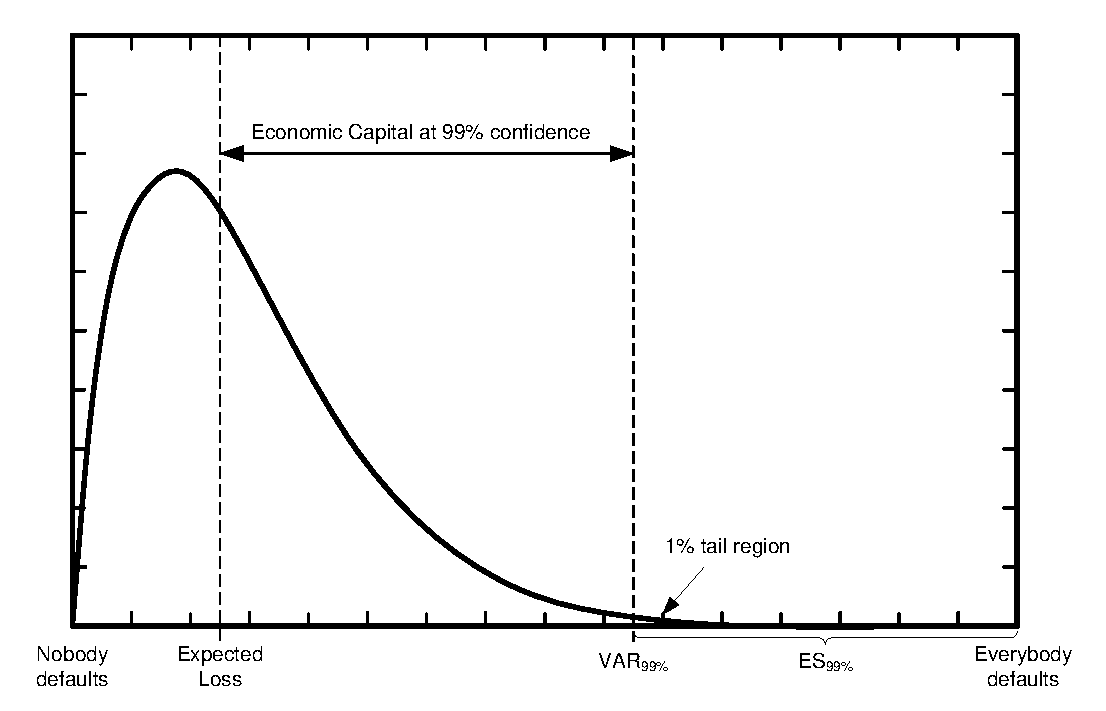
\includegraphics[width=12cm]{creditvar}
\end{figure}


\section{Basic Concepts}

\begin{definition}[Probability of Default (PD)]
The Probability of Default of the i-th obligor, $\text{PD}_i(t)$
indicates the probability that this obligor defaults in the time 
interval $(0,t]$.
\begin{displaymath}
\text{PD}_i(t) = \Pr\{T_i \le t\} = \Pr\{\text{i-th obligor defaults before $t$ years}\}
\end{displaymath}
where $T_i$ is a random variable that represents the default
time of the i-th obligor. Note that the PD defined in this way 
is the cdf of $T_i$.
\end{definition}

\begin{definition}[Exposure At Default (EAD)]
The Exposure At Default of the j-th asset at time $t$ indicates 
the total amount that bank is exposed if the obligor defaults:
\begin{displaymath}
\text{EAD}_j(t) = \left\{
\begin{array}{c}
\text{amount in risk of the j-th asset if the obligor} \\
\text{defaults at time $t$, measured in currency}
\end{array}
\right\}
\end{displaymath}
EAD can be a function dependent of time when these amounts are
fixed and know in advance (eg. loan), or can be a distribution
defined over time when we have a model that support it 
(eg. line of credit).
\end{definition}

\begin{definition}[Loss Given Default (LGD)]
The Loss Given Default of the j-th asset at time $t$ indicates 
the percentage of efective loss over the total exposure:
\begin{displaymath}
\text{LGD}_j(t) = \left\{
\begin{array}{c}
\text{percentage of the $\text{EAD}_j(t)$ that is definitively} \\
\text{lost if the obligor defaults at time $t$}
\end{array}
\right\}
\end{displaymath}
LGD can be a function dependent of time, or can be a distribution
defined over time when we have a model that support it.
\end{definition}

\begin{example}[Bond]
Let a 10-years fixed rate bond with an annual coupon of the
$4\%$ issued by a company rated BB on 01/01/2012. The credit
rating agency reports the PD over time displayed below for this
obligor and rating. The EAD of this asset can be obtained from
its expected cashflow known in advance. We supose that the bank
internal models indicate that in this case the LGD is a 
$\text{Beta}(5,2)$ distribution regardless of the default time.
\begin{figure}[h]
\centering
\subfloat[Probability of Default]{
    \includegraphics[width=7cm]{bond_pd1}
}
\subfloat[Probability of Default (zoom)]{
    \includegraphics[width=7cm]{bond_pd2}
}
\\
\subfloat[Exposure At Default]{
    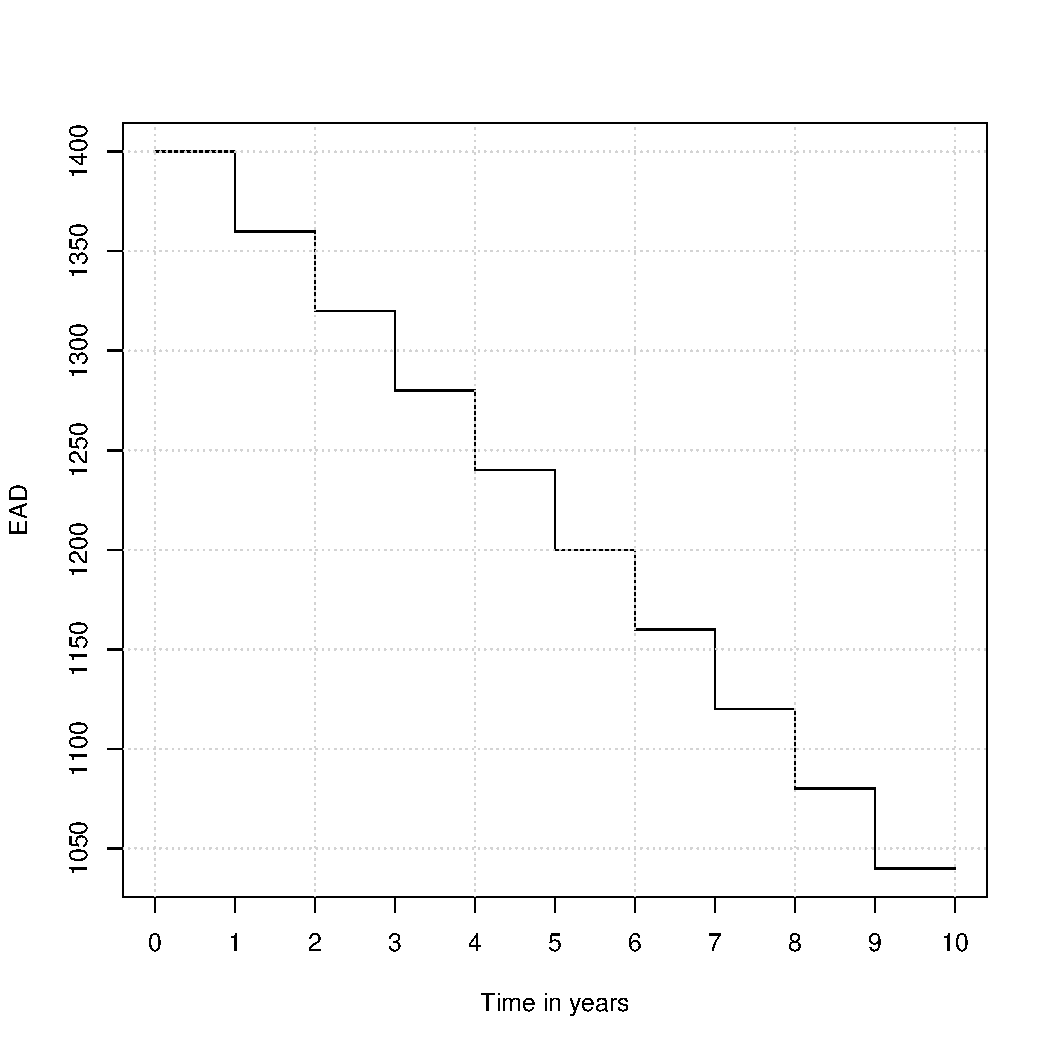
\includegraphics[width=7cm]{bond_ead}
}
\subfloat[Loss Given Default]{
    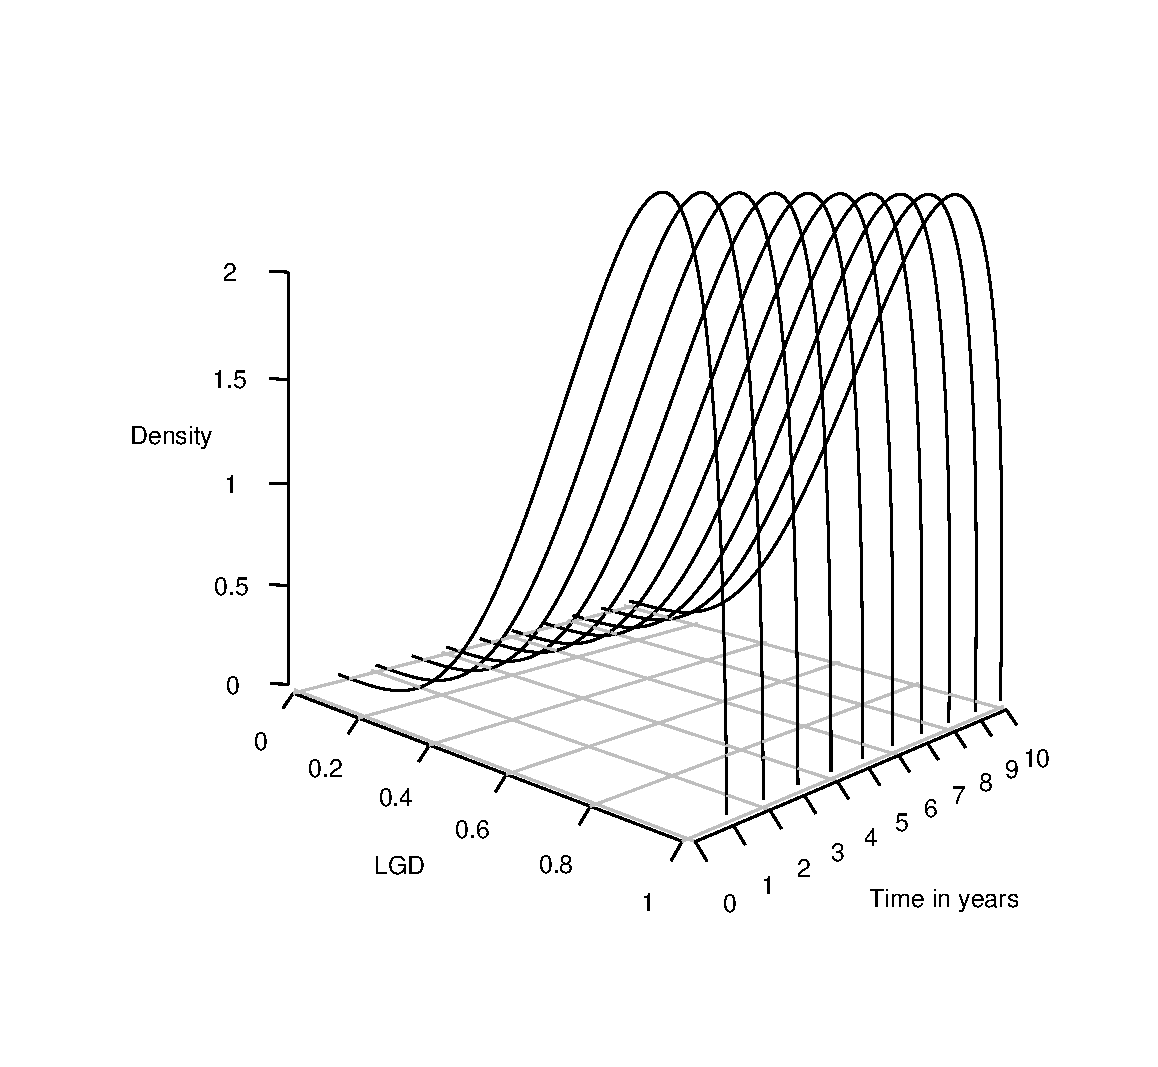
\includegraphics[width=7cm]{bond_lgd}
}
\end{figure}
\end{example}


\cite{mcneil:2005}, \cite{sklar:1959}, \cite{li:2000}, 
\cite{roncalli:2001}, \cite{embrechts:2002}, \cite{cmetrics:1997}
\cite{ntzoufras:2009}, \cite{gordy:2002}, \cite{nagpal:2001}
\cite{meissner:2006}, \cite{bis:2006}

%----------------------------------------------------------------------------------------
% MODEL
%----------------------------------------------------------------------------------------
\chapter{Modeling Default Times}

\section{Mathematics}\index{Mathematics}

\subsection{t-Student Distribution}\index{Mathematics!t-Student Distribution}

\begin{definition}[Multivariate t-Student distribution]
	The $d$-dimensional random vector $X=(X_1,\dots,X_d)$ is said to have a 
	(non-singular) multivariate t-Student distribution with $\nu$ degrees of freedom, 
	mean vector $\mu$ and positive-definite dispersion or scatter matrix $\Sigma$, 
	denoted $t \sim t_d(\nu,\mu,\Sigma)$, if its density is given by
	\begin{displaymath}
		f(x)=\frac{\Gamma\left(\frac{\nu+d}{2}\right)}{\Gamma\left(\frac{\nu}{2}\right)\sqrt{(\pi \nu)^d |\Sigma|}}
		\left(
		1+ \frac{(x-\mu)^\top\Sigma^{-1}(x-\mu)}{\nu}
		\right)^{-\frac{\nu+d}{2}}
	\end{displaymath}
	\noindent where $\Gamma$ is the gamma function, and $|\Sigma|$ is the 
	determinant of the matrix.
\end{definition}

\begin{proposition}[Gaussian as limit of the t-Student]
	The t-Student distribution converges to a Gaussian distribution 
	when $\nu$ tend to $\infty$.
	\begin{displaymath}
		\lim_{\nu \to \infty} t_d(\nu,\mu,\Sigma) = N(\mu,\Sigma)
	\end{displaymath}
\end{proposition}

\begin{proposition}[Multivariate t-Student characterization]
	\label{prop:mtschar}
	A random vector $T \sim t_d(\nu,\mu,\Sigma)$ can be expresed as:
	\begin{displaymath}
		T \stackrel{d}{=} \mu + \sqrt{\frac{\nu}{V}}\cdot Z
		\quad \text{ where } Z \sim N(0,\Sigma) \text{ and } V \sim \chi_{\nu}^2
	\end{displaymath}
\end{proposition}

\begin{proposition}[Multivariate t-Student marginals]
	Let $X \sim t_d(\nu,\vec{0},\Sigma)$. Then, its i-th marginal is 
	$X_i \sim t_1(\nu,0,R_{ii})$.
\end{proposition}

\subsection{t-Student Copula}\index{Mathematics!t-Student Copula}

It is common to use correlation as a measure of dependency between random 
variables. In most cases, this measure does not fully reflect the structure 
of dependence between them. The mathematical concept that does reflect the 
structure of dependence between random variables, however, is the copula, 
which we define below \cite{mcneil:2005}.

\begin{definition}[Copula]
	A copula function, $C$, is a multivariate distribution defined on the 
	unit hypercube $[0,1]^d$ with standard uniform marginals. 
	More precisely,
	\begin{displaymath}
		C(u_1, \dots, u_d) = Pr\{U_1 \le u_1, \dots, U_d \le u_d\}
	\end{displaymath}
	where $U_i \sim \text{Uniform}(0,1) \text{ for } i = 1,\dots, d$.
\end{definition}

Sklar's theorem \cite{sklar:1959} states that any multivariate 
distribution with continuous marginals can be decomposed into the marginals and 
a copula that reflects the structure of dependence between them. Later, we will 
use this statement to define and simulate the t-Student copula.

%%TODO: POSAR REFERENCIA
\begin{theorem}[Sklar's theorem]
	Let $F$ be an $d$-dimensional distribution function with margins $F_1,\dots,F_d$.
	Then there exists an $d$-copula $C$ such that for all $x \in \mathbb{R}^d$,
	\begin{displaymath}
		F(x_1,\dots,x_d) = C(F_1(x_1),\dots,F_d(x_d))
	\end{displaymath}
	If $F_1,\dots,F_d$ are all continuous, the $C$ is unique; otherwise $C$ is uniquely
	determined on $\text{Ran}F_1 \times \dots \times \text{Ran}F_d$.
	Conversely, if $C$ is an $d$-copula and $F_1,\dots,F_d$ are distributions functions,
	then the function $F$ defined above is an $d$-dimensional distribution function
	with margins $F_1,\dots,F_d$.
\end{theorem}

\begin{corollary}[Copula of a multivariate distribution]
	\label{cor:cop1}
	Let $X=(X_1, \dots, X_d)$ a random vector with a multivariate 
	distribution $F$ and continuous marginals $F_1, \dots, F_n$. 
	Then its copula is:
	\begin{displaymath}
		C(u_1,\dots,u_n) = F(F_1^{-1}(u_1), \dots, F_n^{-1}(u_n))
	\end{displaymath}
\end{corollary}
%\begin{proof}
%This is a direct application of Sklar's theorem:
%\begin{displaymath}
%C(F_1(x_1), \dots, F_d(x_d)) = 
%F(F_1^{-1}(F_1(x_1)), \dots, F_d^{-1}(F_d(x_d))) = 
%F(x_1, \dots, x_d)
%\end{displaymath}
%\end{proof}

\begin{corollary}[Copula simulation]
	\label{cor:cop2}
	Let $X=(X_1, \dots, X_d)$ a random vector with a multivariate 
	distribution $F$ and continuous marginals $F_1, \dots, F_n$.
	If we have a procedure to simulate $X$ then we can simulate 
	its copula $C$ using:
	\begin{displaymath}
		(U_1, \dots, U_d) = (F_1(X_1), \dots, F_d(X_d))
	\end{displaymath}
\end{corollary}

\begin{corollary}[Multivariate distribution simulation]
	\label{cor:cop3}
	Let $X=(X_1, \dots, X_d)$ a random vector with a copula $C$
	and continuous marginals $F_1, \dots, F_n$. If we have a
	procedure to simulate $C$ then we can simulate $X$ using:
	\begin{displaymath}
		(X_1, \dots, X_d) = (F_1^{-1}(U_1), \dots, F_d^{-1}(U_d))
	\end{displaymath}
	where $U_i$ are the copula components.
\end{corollary}


\begin{definition}[t-Student copula]
	The t-Student copula, $C_{\nu,\Sigma}^d$, is the copula of the multivariate 
	t-Student distribution $t_d(\nu,\mu,\Sigma)$.
\end{definition}

\begin{proposition}[t-Student copula invariance]
	The copula of $t_d(\nu,\mu,\Sigma)$ is identical of that of $t_d(\nu,\vec{0},R)$
	where $R$ is the correlation matrix implied by the dispersion matrix $\Sigma$.
\end{proposition}

\begin{proposition}[t-Student copula density]
	The t-Student copula, $C_{\nu,R}^d$, where $R$ is a correlation matrix,
	has the following distribution:
	\begin{displaymath}
		C_{\nu,R}^d(u_1, \dots, u_d) = 
		\int_{-\infty}^{t_\nu^{-1}(u_1)} \dots \int_{-\infty}^{t_\nu^{-1}(u_d)} f(x) \ud x
	\end{displaymath}
	where $f(x)$ is the density function of $t_d(\nu,\vec{0},R)$, and $t_{\nu}^{-1}$ 
	denotes the quantile function of the univariate distribution $t_1(\nu,0,1)$. 
	The copula density is
	\begin{displaymath}
		\label{eq:density}
		c_{\nu,R}^d(u_1,\dots,u_d) =
		|R|^{-\frac{1}{2}} 
		\displaystyle\frac{\Gamma{\left(\frac{\nu+d}{2}\right)}}{\Gamma{\left(\frac{\nu}{2}\right)}}
		\displaystyle\left[ \frac{\Gamma{\left(\frac{\nu}{2}\right)}}{\Gamma{\left(\frac{\nu+1}{2}\right)}} \right]^d
		\frac{\displaystyle\left( 1+\frac{\zeta' R^{-1} \zeta}{\nu}\right)^{-\frac{\nu+d}{2}}}{\displaystyle\prod_{i=1}^d \left( 1+\frac{\zeta_i^2}{\nu} \right)^{-\frac{\nu+1}{2}}}
	\end{displaymath}
	\noindent
	where $\zeta=(t_\nu^{-1}(u_1), \dots, t_\nu^{-1}(u_n))$ is the vector of 
	the t-student univariate inverse distribution functions.
\end{proposition}


\subsection{Covariance Block Matrix}\index{Mathematics!Covariance Block Matrix}

\begin{definition}[Covariance Block Matrix]
	We say that a matrix $A$ is a covariance block matrix $B_k(n,d,M)$ where:
	\begin{itemize}
		\item $n=(n_1,\dots,n_k)$ with $n_i \in \mathbb{N}$ and $1 \le n_i$ (number of elements per block),
		\item $d=(d_1,\dots,d_k)$ with $d_i \in \mathbb{R}$ (diagonal block values), and
		\item $M$ is a $k \times k$ symmetric matrix with values $m_{ij} \in \mathbb{R}$ (block values).
	\end{itemize}
	when
	\begin{itemize}
		\item each block $B_{ij}$ is a $n_i \times n_j$ constant matrix with value $M_{ij}$
		\item diagonal blocks $B_{ii}$ have diagonal values $d_i$
		\item A is definite-positive
	\end{itemize}
\end{definition}

\begin{example}[Correlation Block Matrix]
	\label{example1}
	We have $6$ obligors sorted by sector. The first three belong to the 
	banking sector, the next two belong to the energy sector 
	and the last one belongs to the services sector. The correlations are 
	determined by sectors, where $m_{ij}$ is the correlation between two 
	obligors belonging to sectors $i$ and $j$. Then the correlation matrix 
	between obligors is:
	\begin{displaymath}
		R=
		\left(
		\begin{array}{ccc|cc|c} 
			1   & 0.5 & 0.5 & 0.2  & 0.2  & 0.1  \\ 
			0.5 & 1   & 0.5 & 0.2  & 0.2  & 0.1  \\ 
			0.5 & 0.5 & 1   & 0.2  & 0.2  & 0.1  \\ 
			\hline
			0.2 & 0.2 & 0.2 & 1    & 0.4  & 0.15 \\ 
			0.2 & 0.2 & 0.2 & 0.4  & 1    & 0.15 \\ 
			\hline
			0.1 & 0.1 & 0.1 & 0.15 & 0.15 & 1    
		\end{array} 
		\right)
	\end{displaymath}
\end{example}

\begin{proposition}[Covariance block matrix eigenvalues]
	\label{prop1}
	Let $A = B_k(n, d, M)$ a non-singular matrix, and let $G$ be the $k \times k$ 
	deflated matrix
	\begin{displaymath}
		G =
		\left( \begin{array}{cccc}
		d_1+(n_1-1)\cdot m_{11} & n_2 \cdot m_{12}        & \dots  & n_k \cdot m_{1k} \\
		n_1\cdot m_{21}         & d_2+(n_2-1)\cdot m_{22} & \dots  & n_k \cdot m_{2k} \\
		\vdots                  & \vdots                  & \ddots & \vdots \\
		n_1\cdot m_{k1}         & n_2 \cdot m_{k2}        & \dots  & d_k+(n_k-1)\cdot m_{kk} \\
		\end{array} \right)
	\end{displaymath}
	Then, the eigenvalues of $A$ are as follows:
	\begin{itemize}
		\item $d_{r}-m_{rr}$ with multiplicity $n_r-1$ for $r=1,\dots,k$.
		\item $\lambda_r$, the eigenvalues of $G$ with multiplicity $1$.
	\end{itemize}
\end{proposition}

\begin{corollary}
	A covariance block matrix $B_k(n,d,M)$ is definite-positive if
	\begin{itemize}
		\item $d_r > m_{rr}$ for all $r=1,\dots,k$, and
		\item the deflated matrix $G$ is definite-positive.
	\end{itemize}
\end{corollary}


\section{Default Times Distribution}\index{Default Times Distribution}

We assume that obligors default times $(T_1, \dots, T_n)$ are modeled 
by a multivariate distribution $F$ such that:
\begin{displaymath}
	F(t_1, \dots, t_n) = \Pr \{T_1 \le t_1, \dots, T_n \le t_n\}
\end{displaymath}
where $n$ is the number of obligors in the portfolio, $T_i$ is the time 
(in years) when the i-th obligor defaults, and $F$ is the multivariate
distribution. Applying the Sklar's theorem to the above distribution 
we obtain:
\begin{displaymath}
	F(t_1, \dots, t_n) = C\left(F_1(t_1), \dots, F_n(t_n)\right) 
\end{displaymath}
where $F_i(t) = \Pr\{T_i < t\}$ are the marginal distributions, 
and $C$ is the underlying copula.

\subsection{Default Times Marginals}\index{Default Times Distribution!Default Times Marginals}

Marginal distributions are the individual probabilities of default 
(PD) over time. Each obligor has its own PD depending on its rating,
sector, etc. In the following section we infere the PD over time from 
the transition matrix. This approach implies that transition 
probabilities remains contants over time undermining the economic 
cicle effect. In practice, it is equivalent to consider an averaged 
economic cicle.

\begin{definition}[Transition matrix] 
	The $T$-years transition matrix gives the probability of changing 
	from rating $r_i$ to rating $r_j$ in a period of $T$ years:
	\begin{displaymath}
		M_T = \left(
		\begin{array}{ccc}
			m_{1,1} & \dots  & m_{1,n} \\
			\vdots  & \ddots & \vdots  \\
			m_{n,1} & \dots  & m_{n,n} \\
		\end{array}
		\right)
		\qquad
		m_{i,j} = P(r_i \to r_j;T)
	\end{displaymath}
	where $n$ is the number of ratings and $m_{i,j}$ is the probability that a
	obligor with rating $r_i$ changes to rating $r_j$ in $T$ years.
\end{definition}

\begin{example}
	The following table shows a transition matrix in which the probability that 
	a obligor with rating $AA$ changes to rating $B$ in one year is $0.14\%$.
	Note that last column contains the 1-year default probabilities for each 
	rating, and the last row corresponds to the \emph{defaulted} rating.
	
	\begin{figure}[!hb]
		\begin{center}
			\begin{tabular}[]{l|rrrrrrrr}
				        & AAA     & AA      & A       & BBB     & BB      & B                  & CCC     & Default  \\
				\hline
				AAA     & $90.81$ & $8.33$  & $0.68$  & $0.06$  & $0.12$  & $0.00$             & $0.00$  & $0.00$   \\
				AA      & $0.70$  & $90.65$ & $7.79$  & $0.64$  & $0.06$  & $\underline{0.14}$ & $0.02$  & $0.00$   \\
				A       & $0.09$  & $2.27$  & $91.05$ & $5.52$  & $0.74$  & $0.26$             & $0.01$  & $0.06$   \\
				BBB     & $0.02$  & $0.33$  & $5.95$  & $86.93$ & $5.30$  & $1.17$             & $0.12$  & $0.18$   \\
				BB      & $0.03$  & $0.14$  & $0.67$  & $7.73$  & $80.53$ & $8.84$             & $1.00$  & $1.06$   \\
				B       & $0.00$  & $0.11$  & $0.24$  & $0.43$  & $6.48$  & $83.46$            & $4.07$  & $5.21$   \\
				CCC     & $0.22$  & $0.00$  & $0.22$  & $1.30$  & $2.38$  & $11.24$            & $64.86$ & $19.78$  \\
				Default & $0.00$  & $0.00$  & $0.00$  & $0.00$  & $0.00$  & $0.00$             & $0.00$  & $100.00$ \\
			\end{tabular}
			\caption{One-year transition matrix}
			\label{tmatrix1}
		\end{center}
	\end{figure}
\end{example}

\begin{proposition}[Scaled transition matrix]
	The transition matrix can be scaled in time by using the following rules:
	\begin{equation}
		\label{sttm}
		\begin{array}{l}
			M_{T_1+T_2} = M_{T_1} \cdot M_{T_2} \nonumber \\
			M_{k \cdot T} = M_{T}^k \nonumber             \\
			M_{\frac{T}{k}} = \sqrt[k]{M_{T}} \nonumber   
		\end{array}
	\end{equation}
\end{proposition}

The root of a matrix $M$ can be obtained using the spectral decomposition
$M = P \cdot D \cdot P^{-1}$, where $P$ and $D$ are the eigenvectors and
eigenvalues matrices of $M$, doing $M^{\gamma} = P \cdot D^{\gamma} \cdot P^{-1}$

Sometimes, the scaled transition matrix does not satisfy the Markov conditions
(the row sum is equal to one, and all elements are non-negatives). In this case, 
we need to transform this matrix to the relevant Markov matrix. This process is 
called regularization. Below is exposed the QOM regularization algorithm 
extracted from XXX.

\begin{algorithm}[Transition matrix regularization]
	The QOM (Quasi-Optimization of the root Matrix) algorithm regularizes a 
	transition matrix, $m_{ij}$, of dimension $n$ row by row. The steps to 
	regularize the $i$-th row are:
	\begin{enumerate}
		\item Compute the difference between the row sum and one. 
		Divide by $n$ and subtract this value from all non-zero components:
		\begin{displaymath}
			m_{ij} \ne 0 
			\Longrightarrow 
			m_{ij} = m_{ij} - \frac{1}{n} \left( \sum_{j=1}^{n} m_{ij} - 1\right)
		\end{displaymath}
		\item If all the row elements are non-negative and sum to one, 
		then stop, as the row is regularized.
		\item Fix any negative row element to zero and go to Step 1.
	\end{enumerate}
	
	Apply the previous algorithm for every row. The algorithm stops after $m$ 
	steps, where $m \le n$ (Merkoulovitch 2000). The final matrix is a regularized
	matrix. 
\end{algorithm}


\begin{proposition}[PD over time derived from transition matrix]
	Let $M_T$ a transition matrix, then the PD over time, or marginal default
	time distribution, for an obligor with rating $r_j$ is:
	\begin{displaymath}
		\Pr\{T_. \le t\} = \left( M_t \right)_{j, n}
	\end{displaymath}
	where $T_.$ is the obligor default time, $j$ is the index of the obligor's
	rating, $M_t$ is the transition matrix scaled to time $t$, and $n$ is the 
	index of the \emph{defaulted} rating, $r_n$.
\end{proposition}

In some circumstances there is no transition matrix but it is only available
a single value representing the T-period PD of each rating, $p_i$. In these 
cases we can considerer the following diagonal transition matrix:
\begin{displaymath}
	M_T = \left(
	\begin{array}{cccc}
		1-p_1  & \dots  & 0         & p_1     \\
		\vdots & \ddots & \vdots    & \vdots  \\
		0      & \dots  & 1-p_{n-1} & p_{n-1} \\
		0      & \dots  & 0         & 1       \\
	\end{array}
	\right)
\end{displaymath}
This case is equivalent to considere that the PD over time, or marginal default
time distribution, for an obligor with rating $r_j$ is an exponential 
distribution:
\begin{displaymath}
	\Pr\{T_. \le t\} = 1 - e^{-\lambda t} 
	\quad \text{ where } \lambda = -\ln(1-p_j)
\end{displaymath}


\subsection{Default Times Copula}\index{Default Times Distribution!Default Times Copula}

There are several proposals on the copula of the default times
distribution such as the Gaussian copula, the t-Student copula, 
the double-t copula or the Clayton copula [15]. We select the
t-Student copula for the following reasons:

\begin{itemize}
	\item because it is an elliptical copula it is determined by the correlation matrix [??].
	\item because it is an elliptical copula it is symmetrical, allowing to 
	apply the antithetic reduction variance technique in the Monte Carlo 
	simulation.
	\item allows a wide range of dependence structures through parameter $\nu$.
	\item when $\nu \ne \infty$ it exhibits tail dependence.
	\item exist a simulation algorithm easy to implement for higher dimensions.
	\item the Gaussiana case ($\nu = \infty$) is the implicit copula used by 
	CreditMetrics\texttrademark, the de-facto standard.
	\item it is the underlying copula in the multi-factor model.
\end{itemize}

We assume that exist a reduced number $k$ of industrial sectors and that
each obligor belong to a unique sector. Default times dependence between 
obligors only depends on the involved industrials sectors. With these
assumptions, if we sort the obligors by sector, the default times
correlation matrix $R$ is a matrix composed by blocks with $1$'s in the 
diagonal.
\begin{displaymath}
	R =
	\left(
	\begin{array}{ccccccc}
		1          & \dots  & \rho_{1,1} &        & \rho_{1,m} & \dots  & \rho_{1,m} \\
		\vdots     & \ddots & \vdots     & \dots  & \vdots     &        & \vdots     \\
		\rho_{1,1} & \dots  & 1          &        & \rho_{1,m} & \dots  & \rho_{1,m} \\
		
		           & \vdots &            & \ddots &            & \vdots &            \\
		
		\rho_{1,m} & \dots  & \rho_{1,m} &        & 1          & \dots  & \rho_{m,m} \\
		\vdots     &        & \vdots     & \dots  & \vdots     & \ddots & \vdots     \\
		\rho_{1,m} & \dots  & \rho_{1,m} &        & \rho_{m,m} & \dots  & 1          \\
	\end{array}
	\right)
\end{displaymath}

Work directly with the t-Student copula is not practical. For this reason 
we express the distribution of default times according to the Student-t 
distribution instead of the t-Student copula.

\begin{proposition}[Default Times Distribution]
	\label{prop:dtd}
	Let $T=(T_1,\dots,T_n)$ the obligors default times with a t-Student copula 
	$C_{\nu,R}^d$, and marginals $F_i$. 
	Then, the default times distribution $F$ is:
	\begin{displaymath}
		F(t_1,\dots,t_n) = H\left(t_\nu^{-1}(F_1(t_1)), \dots, t_\nu^{-1}(F_n(t_n))\right)
	\end{displaymath}
	where $F$ is the cdf of the multivariate default times, $H$ is the cdf of 
	the multivariate t-Student distribution $t_d(\nu,0,R)$, $t_\nu^{-1}$ is the 
	inverse of the univariate t-Student distribution $t_1(\nu,0,1)$, and $F_i$ 
	is the default probabilities over time of the i-th obligor.
\end{proposition}
\begin{proof}
	We note as $X=(X_1,\dots,X_n)$ a vector having a multivariate t-Student
	distribution $t_{\nu,R}^d$, and we use $(U_1,\dots,U_n)$ to represent
	the components of the copula $C_{\nu,R}^d$.
	\begin{displaymath}
		\begin{array}{rl}
			F(t_1,\dots,t_n) = & \Pr\{ T_1 \le t_1 , \dots, T_n \le t_n \} =                                    \\
			                   & \text{we use the corollary \ref{cor:cop3}: }                                   
			(T_1,\dots,T_n) = (F_1^{-1}(U_1),\dots,F_n^{-1}(U_n)) \\
			=                  & \Pr\{ F_1^{-1}(U_1) \le t_1 , \dots , F_n^{-1}(U_n) \le t_n \} =               \\
			                   & \text{we use the corollary \ref{cor:cop2}: }                                   
			(U_1,\dots,U_n) = (t_\nu(X_1),\dots,t_\nu(X_n)) \\
			=                  & \Pr\{ F_1^{-1}(t_\nu(X_1)) \le t_1 , \dots , F_n^{-1}(t_\nu(X_n)) \le t_n \} = \\
			=                  & \Pr\{ t_\nu(X_1) \le F_1(t_1) , \dots , t_\nu(X_n) \le F_n(t_n) \} =           \\
			=                  & \Pr\{ X_1 \le t_\nu^{-1}(F_1(t_1)) , \dots , X_n \le t_\nu^{-1}(F_n(t_n)) \} = \\
			=                  & H(t_\nu^{-1}(F_1(t_1)), \dots, t_\nu^{-1}(F_n(t_n)))                           \\
		\end{array}
	\end{displaymath}
\end{proof}

Working with the multivariate t-Student distribution with a correlation
matrix of dimension $n \times n$ is not practical to simulate it or for
estimate the parameters. For this reasons we introduce the multi-factor 
models.

\begin{definition}[Gaussian multi-factor model]
	We say that a multivariate distribution $X$ follows a Gaussian multi-factor
	model if it can be expressed in the form:
	\begin{displaymath}
		X_i^j = w_i \cdot Z_i + \sqrt{1-w_i^2} \cdot \epsilon_i^j
		\quad \text{ where } \left\{
		\begin{array}{l}
			i = 1, \dots, k \quad \text{ and $k$ is the number of blocks}    \\
			j = 1, \dots, n_i \quad \text{ and $n_i$ is i-th block size}     \\
			Z \sim N(0,R), \text{ and $R$ a $k \times k$ correlation matrix} \\
			w_i \in (0,1), \text{ are the factor loadings }                  \\
			\epsilon_i^j \sim N(0,1) \text { iid } \forall i,j               \\
			Z, \epsilon_i^j \text{ independents } \forall i,j                \\
		\end{array}
		\right.
	\end{displaymath}
\end{definition}

\begin{proposition}[The Gaussian multi-factor model is a Gaussian distribution]
	\label{prop:gmfigs}
	The Gaussian multi-factor model defined by factor loadings 
	$w_1,\dots,w_k$, the $k \times k$ correlation matrix $R$, and
	$n_1,\dots,n_k$ with $\sum_{i=1}^k n_i = n$ is a 
	multivariate Gaussian distribution with a $n \times n$ correlation
	matrix $\bar{R}$ composed by blocks with values
	$\bar{R}_{i,j} = w_a \cdot w_b \cdot R_{a,b}$ where $a$ and $b$ 
	are the blocks of the indexes $i$ and $j$.
\end{proposition}
\begin{proof}
	We check that the correlations between Gaussian multi-factor model
	components is a matrix composed by blocks that fulfill the equivalence.
	\begin{displaymath}
		\begin{array}{rl}
			\text{Var}(X_i^j) =                       &                                                                                                            
			w_i \cdot \text{Var}(Z_i) + (1-w_i^2) \cdot \text{Var}(\epsilon_i^j) +
			2 \cdot w_i \cdot \sqrt{1-w_i^2} \cdot \text{Cov}(Z_i, \epsilon_i^j) \\
			=                                         & w_i + (1-w_i^2) = 1                                                                                        \\
			                                          &                                                                                                            \\
			\text{Cor}(X_{i_1}^{j_1},X_{i_2}^{j_2}) = & \text{Cov}(X_{i_1}^{j_1},X_{i_2}^{j_2})                                                                    \\
			=                                         & w_{i_1} \cdot w_{i_2} \cdot \text{Cov}(Z_{i_1},Z_{i_2}) +                                                  \\
			                                          & + w_{i_1} \cdot \sqrt{1-w_{i_2}^2} \cdot \text{Cov}(Z_{i_1}, \epsilon_{i_2}^{j_2}) +                       \\
			                                          & + \sqrt{1-w_{i_1}^2} \cdot w_{i_2} \cdot \text{Cov}(Z_{i_2}, \epsilon_{i_1}^{j_1}) +                       \\
			                                          & + \sqrt{1-w_{i_1}^2} \cdot \sqrt{1-w_{i_2}^2} \cdot \text{Cov}(\epsilon_{i_1}^{j_1}, \epsilon_{i_2}^{j_2}) \\
			=                                         & w_{i_1} \cdot w_{i_2} \cdot \text{Cov}(Z_{i_1}, Z_{i_2})                                                   \\
			=                                         & w_{i_1} \cdot w_{i_2} \cdot R_{i_1,i_2}                                                                    \\
		\end{array}
	\end{displaymath}
	The caracterization of the multivariate Gaussian [31, thm 2.6.2]
	states that if every linear combination of the components of a 
	vector $X$ is normally distributed, then $X$ is normally distributed.
	It is straightforward to check that the multi-factor Gaussian model 
	fulfills this property and consequently it is a multivariate Normal.
\end{proof}

\begin{proposition}[Gaussian multi-factor model $\subsetneq$ multivariate Gaussian block]
	Any multi-factor model can be expressed as a multivariate normal 
	block, but there are multivariate normal block that can not be 
	expressed as a Gaussian multi-factor model.
\end{proposition}
\begin{proof}
	Proposition \ref{prop:gmfigs} states that any multi-factor model 
	can be expressed as a multivariate normal composed by blocks.
	Next we see that reciprocal is false. We use the equivalence 
	$\bar{R}_{i,j} = w_a \cdot w_b \cdot R_{a,b}$ between
	the multi-factor correlation matrix $R$ and the multivariate block
	Gaussian correlation matrix $\bar{R}$.
	
	\textbf{Counterexample 1}. Factor loading with imaginary value.
	\begin{displaymath}
		\bar{R} = \left(
		\begin{array}{cc|c}
			1    & -0.5 & 0 \\
			-0.5 & 1    & 0 \\
			\hline
			0    & 0    & 1 \\
		\end{array}
		\right) 
		\longrightarrow
		R = \left(
		\begin{array}{cc}
			1 & 0 \\
			0 & 1 \\
		\end{array}
		\right)
		\text{ , }
		w = (\sqrt{-0.5}, 1)
		\text{ !!}
	\end{displaymath}
	
	\textbf{Counterexample 2}. Correlation with absolute value > 1.
	\begin{displaymath}
		\bar{R} = \left(
		\begin{array}{cc|cc}
			1   & 0.5 & 0.6 & 0.6 \\
			0.5 & 1   & 0.6 & 0.6 \\
			\hline
			0.6 & 0.6 & 1   & 0.5 \\
			0.6 & 0.6 & 0.5 & 1   \\
		\end{array}
		\right) 
		\longrightarrow
		R = \left(
		\begin{array}{cc}
			1               & \frac{0.6}{0.5} \\
			\frac{0.6}{0.5} & 1               \\
		\end{array}
		\right)
		\text{ , }
		w = (\sqrt{0.5}, \sqrt{0.5})
		\text{ !!}
	\end{displaymath}
\end{proof}

It's disturbing that exist multivariate block Gaussian distributions 
that can't be expressed as a multi-factor model. Fortunately the 
cases where that ocurre haven't practical interest in credit risk
modeling where the number of obligors in each block are higher. 
The following proposition clarifies this theme.

\begin{proposition}[Gaussian multi-factor model $\approx$ multivariate Gaussian block]
	\label{prop:gmfamgb}
	Let $X \sim N(0,\bar{R})$ with $\bar{R}$ a correlation block matrix 
	$B_2(n,\vec{1},M)$. Then $X$ can be expressed as a multi-factor 
	Gaussian model if $n_1$ and $n_2$ are large enough.
\end{proposition}
\begin{proof}
	We use the proposition \ref{prop1} to prove the statement Usamos la caracterización de las matrices de covarianzas por bloques (Simulation of High-Dimensional t-Student Copulas, Gerard Torrent-Gironella and Josep Fortiana) PONER REFERENCIA para demostrar la proposición en los dos casos posibles.
	
	\textbf{Case 1}. Factor loading $w_i$ with imaginary value is caused by a negative 
	$m_{ii}$ value ($m_{ii} = w_i^2$). We use the proposition \ref{prop1} to determine
	the restrictions about $m_{ii}$. Because $\bar{R}$ is covariance block matrix 
	definite-positive, the deflated matrix has a positive determinant. Then,
	\begin{displaymath}
		\begin{array}{l}
			1 + (n_1-1) \cdot m_{11} + (n_2-1) \cdot m_{22} +                     
			(n_1-1) \cdot (n_2-1) \cdot m_{11} \cdot m_{22} -                     
			n_1 \cdot n_2 \cdot m_{12}^2 > 0                                      
			                                                                      \\
			m_{11} > \frac{n_1 \cdot n_2 \cdot m_{12}^2 -1 -(n_2-1) \cdot m_{22}} 
			{(n_1-1) + (n_1-1) \cdot (n_2-1) \cdot m_{11}}                        
			                                                                      \\
			\text{tending } n_1 \to \infty                                        
			                                                                      \\
			m_{11} \ge 0                                                          
		\end{array}
	\end{displaymath}
	
	\textbf{Case 2}. Multi-factor model correlation bigger than $1$ is caused
	by $m_{12} = w_1 \cdot w_2 \cdot R_{12} = \sqrt{m_{11}} \cdot \sqrt{m_{22}} \cdot R_{12}$
	causing $R_{12} = \frac{m_{12}}{\sqrt{m_{11} \cdot m_{22}}}$.
	\begin{displaymath}
		\begin{array}{l}
			1 + (n_1-1) \cdot m_{11} + (n_2-1) \cdot m_{22} +                     
			(n_1-1) \cdot (n_2-1) \cdot m_{11} \cdot m_{22} -                     
			n_1 \cdot n_2 \cdot m_{12}^2 > 0                                      
			                                                                      \\
			m_{12}^2 <                                                            
			\frac{1}{n_1 \cdot n_2} +                                             
			\frac{(n_1-1)}{n_1 \cdot n_2} \cdot m_{11} +                          
			\frac{(n_2-1)}{n_1 \cdot n_2} \cdot m_{22} +                          
			\frac{(n_1-1) \cdot (n_2-1)}{n_1 \cdot n_2} \cdot m_{11} \cdot m_{22} 
			                                                                      \\
			\text{tending } n_1 \to \infty \text{ and } n_2 \to \infty            
			                                                                      \\
			m_{12}^2 \le m_{11} \cdot m_{22}                                      
		\end{array}
	\end{displaymath}
\end{proof}

\begin{definition}[t-Student multi-factor model]
	We combine the t-Student characterization (proposition\ref{prop:mtschar})
	and the multivariate Gaussian distribution expressed as a
	Gaussian multi-factor model to define the t-Student multi-factor
	model:
	\begin{displaymath}
		X_i^j = \sqrt{\frac{\nu}{V}} \cdot 
		\left( w_i \cdot Z_i + \sqrt{1-w_i^2} \cdot \epsilon_i^j \right)
		\quad \text{ where } \left\{
		\begin{array}{l}
			i = 1, \dots, k \quad \text{ and $k$ is the number of blocks}    \\
			j = 1, \dots, n_i \quad \text{ and $n_i$ is i-th block size}     \\
			V \sim \chi_{\nu}^2, \quad 2 \le \nu \text{ degrees of freedom}  \\
			Z \sim N(0,R), \text{ and $R$ a $k \times k$ correlation matrix} \\
			w_i \in (0,1), \text{ are the factor loadings }                  \\
			\epsilon_i^j \sim N(0,1) \text { iid } \forall i,j               \\
			V, Z, \epsilon_i^j \text{ independents } \forall i,j             \\
		\end{array}
		\right.
	\end{displaymath}
\end{definition}

By contruction, the t-Student multi-factor model is a multivariate
t-Student distribution with a block correlation matrix. With some
minor exceptions (see proposition \ref{prop:gmfamgb}) we can 
state that any multivariate t-Student distribution can be expressed
as a t-Student multi-factor model.

%----------------------------------------------------------------------------------------
% PARAMETERS ESTIMATION
%----------------------------------------------------------------------------------------
\chapter{Parameters Estimation}

We want to estimate the t-Student multi-factor parameters 
($\nu, w_i, R$). The available information is:
\begin{itemize}
	\item $N_{srt}$ = Number of obligors in sector $s$, rating $r$ and year $t$
	\item $K_{srt}$ = Number of defaults in sector $s$, rating $r$ and year $t$
\end{itemize}


\begin{notation}[1-year threshold]
	We indicate as $p_i$ the probability that i-the obligor defaults in 
	the first period.
	\begin{displaymath}
		p_i = \Pr\{T_i \le 1 \text{ year}\} = F_i(1) 
	\end{displaymath}
\end{notation}

In most cases there is no historical records disaggregated at the rating
level. In these cases, when the historical records are $N_{st}$ and 
$K_{st}$ without the counts by rating, we can use the following approximation:
\begin{displaymath}
	K_{srt} = K_{st} \cdot \frac{p_r}{\displaystyle \sum_{i \ne default} p_i}
\end{displaymath}

%TODO: posar exemple?

\begin{definition}[Annual number of defaults]
	We define the annual number of defaults by sector and rating like a
	discrete multivariate random variable 
	$K=(K_{11}, \dots, K_{1r}, \dots, K_{k1}, \dots, K_{kr})$ where:
	\\
	$K_{ij}$ = number of obligors in the sector $i$ that defaults in a
	period of 1-year having a rating $j$ at the begining of the period.
\end{definition}

\begin{proposition}[Density of the annual number of defaults (I)]
	The density (pdf) of the annual number of defaults, assuming that these
	are distributed according to a multivariate block t-Student distribution
	with $\nu$ degrees of freedom, block correlation matrix $B_k(n,1,M)$, is:
	\begin{displaymath}
		\begin{array}{l}
			K(k_{11},\dots,k_{1r},\dots,k_{k1},\dots,k_{kr}; B_k,\nu) =                                   \\
			                                                                                              \\
			= \Pr\{K_{11}=k_{11},\dots,K_{1r}=k_{1r},\dots,K_{k1}=k_{k1},\dots,K_{kr}=k_{kr}; B_k,\nu\} = \\
			                                                                                              \\
			= \left( \displaystyle \prod_{i=1}^k \prod_{j=1}^r \binom{n_{ij}}{k_{ij}} \right) \cdot       
			\displaystyle                                                                                 
			\underbrace{\int_{-\infty}^{t_{\nu}^{-1}(p_1)}}_{k_{11} \text{ times}}                        
			\underbrace{\int_{t_{\nu}^{-1}(p_1)}^{\infty}}_{n_{11}-k_{11} \text{ times}}                  
			\dots                                                                                         
			\underbrace{\int_{-\infty}^{t_{\nu}^{-1}(p_r)}}_{k_{kr} \text{ times}}                        
			\underbrace{\int_{t_{\nu}^{-1}(p_r)}^{\infty}}_{n_{kr}-k_{kr} \text{ times}}                  
			f(x_1,\dots,x_n) \ud x_1 \dots \ud x_n                                                        
		\end{array}
	\end{displaymath}
	where $n_{ij}$ is the number of obligors in the i-th sector with the 
	j-th rating, $k_{ij}$ is the number of defaults in the i-th sector 
	with the j-th rating, $n = \sum n_{ij}$ is the number of obligor in the
	portfolio, $f()$ is the $t_n(\nu,\bar{R})$ pdf, $t_{\nu}^{-1}$ is the
	inverse of the univariate t-Student cdf. The combinatorial coeficients
	takes in account all the combinations of interchangeable obligors.
\end{proposition}

We don't known an analitical expression for the density of the annual 
number of defaults. For this reason we try to solve the problem recurring 
to the multi-factor formulation.

%TODO: canviar subindex K per S (en el cas de sectors)
\begin{proposition}[Conditioned density of the annual number of defaults]
	The conditioned density (pdf) of the annual number of defaults, assuming 
	that these are distributed according to a t-Student multi-factor model
	with $\nu$ degrees of freedom, factor loadings $w_i$, and correlations
	$R$ is:
	\begin{displaymath}
		\begin{array}{l}
			K(k_{11},\dots,k_{1r},\dots,k_{k1},\dots,k_{kr} | v,z_1,\dots,z_k; \nu, w_1,\dots,w_k, R) =                                   \\
			                                                                                                                              \\
			= \Pr\{K_{11}=k_{11},\dots,K_{1r}=k_{1r},\dots,K_{k1}=k_{k1},\dots,K_{kr}=k_{kr} | v,z_1,\dots,z_k; \nu, w_1,\dots,w_k, R\} = \\
			                                                                                                                              \\
			= \displaystyle \prod_{i=1}^k \prod_{j=1}^r \binom{n_{ij}}{k_{ij}} \cdot
			H_{ij}(v,z_i)^{k_{ij}} \cdot
			\left( 1 - H_{ij}(v,z_i) \right)^{n_{ij}-k_{ij}}
		\end{array}
	\end{displaymath}
	where
	\begin{displaymath}
		H_{sr}(v,z_s) = \phi\left(  
		\frac{\sqrt{\frac{v}{\nu}} \cdot t_{\nu}^{-1}(p_r) - w_s\cdot z_s}{\sqrt{1-w_s^2}}
		\right)
	\end{displaymath}
	and $n_{ij}$ is the number of obligors in the i-th sector with the 
	j-th rating, $k_{ij}$ is the number of defaults in the i-th sector 
	with the j-th rating, $\phi$ is the pdf of the univariate $N(0,1)$
	, and $t_{\nu}^{-1}$ is the inverse of the univariate t-Student cdf. 
	The combinatorial coeficients takes in account all the combinations 
	of interchangeable obligors.
\end{proposition}
\begin{proof}
	Let $H_{sr}$ the probability that an obligor belonging to sector $s$
	with initial rating $r$ defaults conditioned to $z_s$ and $v$.
	We use the pdf of the default times distribution (see proposition 
	\ref{prop:dtd}) to assess it value:
	\begin{displaymath}
		H_{sr} = 
		\Pr\{T_i \le 1; v, z_s\} = 
		\Pr\{ X_i \le t_{\nu}^{-1}(F_i(1)); v, z_s\} = 
		\Pr\{ X_i \le t_{\nu}^{-1}(p_r); v, z_s\}
	\end{displaymath}
	wehre $T_i$ is the i-th component of the multivariate default 
	times, $F_i$ is PD over time of the i-th obligor (that has 
	rating r), and $X_i$ is the i-th component of the multivariate 
	t-Student. Now express $X$ in the multi-factor form:
	\begin{displaymath}
		H_{sr} = \Pr \left\{ 
		\sqrt{\frac{\nu}{v}} \cdot \left( w_s \cdot z_s + \sqrt{1-w_s^2} \cdot \epsilon\right)
		\le t_{\nu}^{-1}(p_r)
		\right\}
	\end{displaymath}
	Because $v$ and $z_s$ are fixed and independent from $\epsilon \sim N(0,1)$, we obtain:
	\begin{displaymath}
		H_{sr}(v,z_s) = \phi\left(  
		\frac{\sqrt{\frac{v}{\nu}} \cdot t_{\nu}^{-1}(p_r) - w_s\cdot z_s}{\sqrt{1-w_s^2}}
		\right)
	\end{displaymath}
	Once the probability of default by one obligor, the probability of 
	observing $k$ failures in a set of $n$ independent obligors follows 
	a binomial distribution:
	\begin{displaymath}
		\text{Bin}(k;n,p) = \binom{n}{k} \cdot p^k \cdot (1-p)^{n-k}
	\end{displaymath}
	The product for all sectors and ratings gives the stated formula. 
	We can do the product because $v$ and $z_s$ are fixed.
\end{proof}

\begin{corollary}[Density of the annual number of defaults (II)]
	We can express the density of the annual number of defaults using 
	the conditioned density:
	\begin{displaymath}
		\begin{array}{l}
			K(k_{11},\dots,k_{1r},\dots,k_{k1},\dots,k_{kr} ; \nu, w_1,\dots,w_k, R) =                \\
			\displaystyle \int_0^{\infty} \int_{\mathbb{R}^k}                                         
			\psi(v) \cdot \phi(z_1,\dots,z_k) \cdot                                                   
			K(k_{11},\dots,k_{1r},\dots,k_{k1},\dots,k_{kr} | v,z_1,\dots,z_k; \nu, w_1,\dots,w_k, R) 
			\ud z_1 \dots \ud z_k \ud v                                                               
		\end{array}
	\end{displaymath}
	where $\psi$ is the $\chi_{\nu}^2$ pdf, and $\phi$ is the $N(0,R)$ pdf.
\end{corollary}

\begin{definition}[Conditioned likelihood]
Let a set of observations $\{K^t, N^t\}_{t=1,\dots,T}$ where $N^t$ 
and $K^t$ are vectors representing the number of obligors and defaulted 
obligors in each sector-rating bucket. We define the conditional 
likelihood of these observations as:
\begin{displaymath}
	\begin{array}{l}
		L(\nu,\vec{w},R | v^1,\vec{z^1},\dots,v^T,\vec{z^T} ; K^1,\dots,K^T) = \\
		\displaystyle \prod_{t=1}^T K(k_{11}^t,\dots,k_{sr}^t | v^t,\vec{z^t}; \nu,\vec{w},R) = \\
		\displaystyle
		\prod_{t=1}^T \prod_{i=1}^s \prod_{j=1}^r 
		\binom{n_{ij}^t}{k_{ij}^t} \cdot
		H_{ij}(v^t,z_i^t)^{k_{ij}^t} \cdot
		\left( 1 - H_{ij}(v^t,z_i^t) \right)^{n_{ij}^t-k_{ij}^t}
	\end{array}
\end{displaymath}
Note that the parameters to be infered are $\nu,\vec{w},R$ and the
latent variables $v^1,\vec{z^1},\dots,v^T,\vec{z^T}$.
\end{definition}

\begin{proposition}[Parameters estimation]
	We can estimate the parameters of the conditioned likelihood using
	the Bayessian framework and Metropolis-Hastings algorithm 
	(see algorithm \ref{alg:bimh}) with the following rules:
	\begin{itemize}
		\item parameters $\theta \equiv \{ \nu,w_1,\dots,w_k,R,v^1,\vec{z^1},\dots,v^T,\vec{z^T}\}$
		\item observations $y \equiv \{K^t, N^t\}_{t=1,\dots,T}$
		\item likelihood $f(y|\theta) \equiv L(\nu,\vec{w},R | v^1,\vec{z^1},\dots,v^T,\vec{z^T} ; K^1,\dots,K^T)$
		\item proposal distributions $q(\theta_j|\theta_j') \sim N(\theta,\sigma_j)$
		\item prior distribution $f(\nu) \sim \text{Unif}(2,1000)$
		\item prior distribution $f(w_i) \sim \text{Unif}(0,1) \quad i=1,\dots,k$
		\item prior distribution $f(r_{ij}) \sim \Upsilon(\vec{z}^1,\dots,\vec{z}^T,R) \quad i=1,\dots,k, \quad j=(i+1),\dots,k$
		\item prior distribution $f(\vec{z}^t) \sim N(\vec{0},R) \quad t=1,\dots,T$
		\item prior distribution $f(v^t) \sim \chi_{\nu}^2 \quad t=1,\dots,T$
	\end{itemize}
	For the prior distributions of $r_{ij}$ we select the one that 
	maximize the probability to observe the latent variables. The 
	pdf of the distribution $\Upsilon(\vec{z}^1,\dots,\vec{z}^T,R)$ is:
	%hyperparameters, hyperdistributions
	\begin{displaymath}
		f(r_{ij}) = f(r; i,j,R) = \frac
		{\displaystyle \prod_{t=1}^{T} \phi\left( \vec{z}^t; \vec{0}, R(r,i,j) \right)}
		{\displaystyle \int \prod_{t=1}^{T} \phi\left( \vec{z}^t; \vec{0}, R(r,i,j) \right) \ud r}
	\end{displaymath}
	where $\phi$ is the pdf of the multivariate $N(0,R)$ distribution,
	and $R(r,i,j)$ is the matrix $R$ with the cell $(i,j)$ value 
	replaced by $r$. We don't need to know the limits of the integral
	because this is constant and cancels into the M-H algorithm.
\end{proposition}

\begin{proposition}[Robbins-Monro process]
CAL MILLORAR MOLT AIXO. 
proceso de Robbins-Monro tal como se indica en [¿24?].
	\begin{displaymath}
		\sigma_{i+1} = \left\{
		\begin{array}{ll}
			\sigma_i \cdot \left( 1 + \frac{1}{p \cdot i} \right) & \text{if $y$ is accepted} \\
			\sigma_i \cdot \left( 1 - \frac{1}{(1-p) \cdot i} \right) & \text{if $y$ is rejected} \\
		\end{array}
		\right.
	\end{displaymath}
	we take an arbitrary starting value $\sigma_0$.
\end{proposition}

\section{Bayessian Inference}\index{Bayessian Inference}

Bayesian statistics differ from the classical statistical 
theory since all unknown parameters are considered as random 
variables. We want calculate the distribution $f(\theta|y)$ 
of the parameters $\theta$ given the observed data $y$. 
According to the Bayes theorem, this can be written as:
\begin{displaymath}
	f(\theta|y) = \frac{f(y|\theta) \cdot f(\theta)}{f(y)} \propto f(y|\theta) \cdot f(\theta)
\end{displaymath}

We call \emph{posterior distribution} to $f(\theta|y)$ and 
\emph{prior distribution} to $f(y)$. This prior distribution 
expresses the information available to the researcher before 
any data are involved in the statistical analysis. $f(y|\theta)$ 
is the probability of observing $y$ given $\theta$, and is also 
known as the likelihood.
\begin{displaymath}
	f(y|\theta) = \prod_{i=1}^n f(y_i|\theta)
\end{displaymath}


\section{Metropolis-Hastings}\index{Metropolis-Hastings}

\begin{algorithm}[Metropolis-Hastings]
	Let us assume a target distribution $f(x)$ from which we wish to generate a 
	sample of size $T$. The Metropolis-Hastings algorithm can be described by the 
	following iterative steps; where $x^{(t)}$ is the vector of generated values 
	in the $t$-th iteration of the algorithm:
	\begin{enumerate}
		\item Set initial values $x^{(0)}$
		\item For $t=1,\dots,T$ repeat the following steps
		\begin{itemize}
			\item Set $x=x^{(t-1)}$
			\item Let $x'$ a random value from the proposal distribution $q(x \to x’)=q(x'|x)$
			\item Calculate the acceptance rate 
			$\alpha = \min\left(1,\frac{f(x') \cdot q(x|x')}{f(x) \cdot q(x'|x)}\right)$
			\item Update $x^{(t)}=\left\{
			\begin{array}{ll}
				x'        & \text{ with probability } \alpha   \\
				x^{(t-1)} & \text{ with probability } 1-\alpha 
			\end{array}\right.$ 
		\end{itemize}
	\end{enumerate}
\end{algorithm}

%TODO: list ergodic properties
%TODO: referenciar llibre WinBugs


\textbf{Bayesian inference}.
The Metropolis-Hastings algorithm outlined above can be directly implemented to do
Bayesian inference by substituting $x$ by the unknow parameters, $\theta$, and 
the target distribution $f(x)$ by the posterior distribution $f(\theta|y)$. Then 
the acceptance rate becomes:
\begin{displaymath}
	\alpha = \min\left(1,\frac{f(\theta'|y) \cdot q(\theta|\theta')}{f(\theta|y) \cdot q(\theta'|\theta)}\right) = \min\left(1,\frac{f(y|\theta') \cdot f(\theta') \cdot q(\theta|\theta')}{f(y|\theta)  \cdot f(\theta) \cdot q(\theta'|\theta)}\right)
\end{displaymath}


\textbf{Random-walk Metropolis-Hastings} is a special case with symmetric proposals
$q(\theta'|\theta) = q(\theta|\theta')$ where $q(\theta'|\theta) \equiv N(\theta,S)$. 
In this case the acceptance rate depends only on the posterior distribution
and, in the Bayesian inference Metropolis-Hastings case, becomes:
\begin{displaymath}
	\alpha = 
	\min\left(1,\frac{f(y|\theta') \cdot f(\theta') \cdot q(\theta|\theta')}{f(y|\theta)  \cdot f(\theta) \cdot q(\theta'|\theta)}\right) = 
	\min\left(1,\frac{f(y|\theta') \cdot f(\theta')}{f(y|\theta) \cdot f(\theta)}\right)
\end{displaymath}


\textbf{Metropolis-Hastings using logarithms}.
The product of functions involves complicated expressions and accuracy 
problems. For this reason it is usual to operate with logarithms. The 
logarithmic version of the acceptance rate, in the Bayesian inference 
Metropolis-Hastings case, becomes:
\begin{displaymath}
	\ln(\alpha) = \min \left( \ln(1),  
	\ln \left(\frac{f(y|\theta') \cdot f(\theta')}{f(y|\theta) \cdot f(\theta)}\right)
	\right) = 
	\min \left( 0,
	\ln f(y|\theta') + \ln f(\theta') - \ln f(y|\theta) - \ln f(\theta)
	\right)
\end{displaymath}


\textbf{Single-component Metropolis-Hastings} algorithm consist in update sequentially 
univariate components using Metropolis-Hastings steps. 
One generated observation $\theta^{(t)}$ is obtained after updating all 
components of the parameter vector. Generally, the sequence of updating the 
elements of $\theta$ does not influence the convergence of the algorithm.
We use the notation $\theta_{\backslash j}$ to indicate the vector $\theta$ 
excluding its j-th component [ i.e., $\theta_{\backslash j} = 
(\theta_1,\dots,\theta_{j-1},\theta_{j+1},\dots,\theta_{d})$ ].


\begin{algorithm}[Bayesian inference Metropolis-Hastings] \ 
\label{alg:bimh}
	\begin{enumerate}
		\item Set initial values $\theta^{(0)}$
		\item For $t=1,\dots,T$ repeat the following steps
		\begin{itemize}
			\item Set $\theta=\theta^{(t-1)}$
			\item For $j=1,\dots,d$ repeat the following steps
			\begin{enumerate}[label=\alph*.]
				\item $\theta_j' = N(\theta_j,S_j)$
				\item Calculate the logarithm of the acceptance rate \\
				$\ln(\alpha) = \min \left( 0,
				\ln f(y|\theta_j',\theta_{\backslash j}) + 
				\ln f(\theta_j',\theta_{\backslash j}) - 
				\ln f(y|\theta_j,\theta_{\backslash j}) - 
				\ln f(\theta_j,\theta_{\backslash j})
				\right)$
				\item Simulate $u \sim U(0,1)$
				\item Update $\theta_j=\left\{
				\begin{array}{ll}
					\theta_j' & \text{ if } \ln(u) < \ln(\alpha) \\
					\theta_j  & \text{ otherwise }               
				\end{array}\right.$ 
			\end{enumerate}
			\item Set $\theta^{(t)}=\theta$
		\end{itemize}
	\end{enumerate}
\end{algorithm}


%----------------------------------------------------------------------------------------
% MODELING PORTFOLIO LOSS
%----------------------------------------------------------------------------------------
\chapter{Modeling Portfolio Loss}

\section{Portfolio Loss Distribution}

Let a portfolio where we have the obligor default times
$(T_1,\dots,T_n)$ modeled by its PD over time and a
t-Student copula. For each obligor we know its exposure

OLALA

%----------------------------------------------------------------------------------------
%	BIBLIOGRAPHY
%----------------------------------------------------------------------------------------
\chapter*{Bibliography}
\addcontentsline{toc}{chapter}{\textcolor{ocre}{Bibliography}}
% \section*{Books}
% \addcontentsline{toc}{section}{Books}
% \printbibliography[heading=bibempty,type=book]
% \section*{Articles}
% \addcontentsline{toc}{section}{Articles}
% \printbibliography[heading=bibempty,type=article]
% \section*{Others}
% \addcontentsline{toc}{section}{Others}
% \printbibliography[heading=bibempty,type=techreport]

\section*{References}
%\addcontentsline{toc}{section}{References}
\printbibliography[heading=bibempty]

%----------------------------------------------------------------------------------------
%	INDEX
%----------------------------------------------------------------------------------------
\cleardoublepage
\setlength{\columnsep}{0.75cm}
\addcontentsline{toc}{chapter}{\textcolor{ocre}{Index}}
\printindex

%----------------------------------------------------------------------------------------

\end{document}
